Step1: we need to find the solution of equation:\\
\begin{align}
\myvec{2 & -3}\textbf{x} = 4 \label{eqn:solutions/line_plane/601}\\
\myvec{3 & 4}\textbf{x} = 5\label{eqn:solutions/line_plane/602}
\end{align}


\begin{align}
\begin{pmatrix}
    2 & -3 & 4 \\ 
    3 & 4 & 5
\end{pmatrix} \label{eqn:solutions/line_plane/603}
\end{align}
Transforming the matrix into row-echelon form \\
\begin{align}
\myvec{
2 & -3 & 4 \\
3 & 4 & 5\\
}
  \xleftrightarrow[]{R1 \leftarrow \frac{4}{17}*(R1+ \frac{3}{4}R2) } \nonumber \label{eqn:solutions/line_plane/604} \\
\myvec{
1 & 0 & 31/17 \\
3 & 4 & 5
}
\end{align}
\begin{align}
\myvec{
1 & 0 & 31/17 \\
3 & 4 & 5
}
  \xleftrightarrow[]{R2 \leftarrow \frac{1}{4} (R2- 3*R1) } \nonumber \label{eqn:solutions/line_plane/605}  \\
\myvec{
1 & 0 & 31/17 \\
0 & 1 & -2/17
}
\end{align}

After solving this two equation we will get the junction point, which is intersection of this line segments.
Thus, Junction Point is (31/17 \space -2/17)
To reach in the least time, he should follow the shortest path, i.e, perpendicular from the junction point to the line give by this equation:
\begin{align}
\myvec{6 & -7}\textbf{x} = 8 \label{eqn:solutions/line_plane/606}
\end{align}
normal vector to the given line is:
\begin{align}
\vec{n}=\myvec{0 & -1\\ 1 & 0}\myvec{6 \\ -7}\label{eqn:solutions/line_plane/607}\\
\vec{n}=\myvec{7\\6}  \label{eqn:solutions/line_plane/608} 
\end{align}

\begin{figure}[!htbp]
\centering 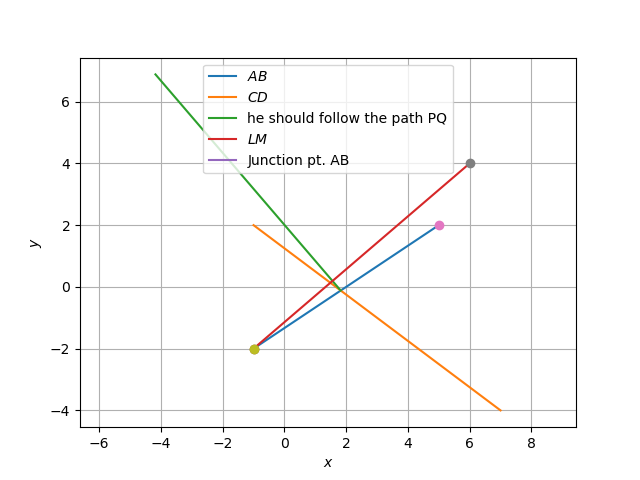
\includegraphics[width=\columnwidth]{./solutions/line_plane/60/Figure_1.png}
\caption{The Required path is PQ.}
\label{fig:solutions/line_plane/60/ Path PQ}
\end{figure}

The equation of the line in terms of normal vector passing through a given point is obtained as\\
\begin{align}
\vec{n}^T(\vec{x}-\vec{A})=0 \label{eqn:solutions/line_plane/609} \\
\vec{n}^T\vec{x}=\vec{n}^T\vec{A} \label{eqn:solutions/line_plane/6010}
\end{align}
Hence, he should follow this path PQ:
\begin{align}
\myvec{7 & 6} \textbf{x} = \frac{205}{17}\label{eqn:solutions/line_plane/6011}
\end{align}



